\section{Additional Experiments}










\subsection{Training Cost and Practicality Analysis}
\label{app:cost}

A natural concern is whether the step-wise divergence computation in \ourmodel introduces substantial overhead relative to standard OPD. We address this by reporting wall-clock training metrics for all methods. All experiments are conducted on 8$\times$H20 GPUs with identical batch sizes and rollout configurations, trained for 120 steps (0.6B) or 150 steps (1.7B). Key observations are summarized as:

\begin{table}[h]
    \centering
    \caption{
    Training cost comparison. All runs use 8$\times$H20 96GB GPUs with identical configurations.}
    \vspace{0.4 em}
    \label{tab:cost}

    \begingroup
    \setlength{\tabcolsep}{4pt}
    \renewcommand{\arraystretch}{1.08}
    \normalsize

    \begin{adjustbox}{max width=0.76\textwidth}
    \begin{tabular}{llccc}
        \toprule
        \multirow{2}{*}{\textbf{Params}} 
        & \multirow{2}{*}{\textbf{Method}} 
        & \textbf{Avg Time/Step} 
        & \textbf{Peak Memory} 
        & \textbf{Total Time} \\
        & & (s) & (GB) & (h) \\

        \midrule
        \multirow{3}{*}{\textbf{0.6B}}
        & GRPO 
        & 680.6 & 78.5 & 22.7 \\
        & OPD 
        & 1090.5 & 87.7 & 36.4 \\
        & \ourmodel 
        & 1052.3 & 87.6 & 35.1 \\

        \midrule
        \multirow{3}{*}{\textbf{1.7B}}
        & GRPO 
        & 784.6 & 81.7 & 32.7 \\
        & OPD 
        & 1053.6 & 88.2 & 43.9 \\
        & \ourmodel 
        & 1105.4 & 88.7 & 46.1 \\

        \bottomrule
    \end{tabular}%
    \end{adjustbox}

    \endgroup
    \vspace{-10pt}
\end{table}

\paragraph{SOD vs.\ OPD: negligible algorithmic overhead.}
The step-wise divergence $d_k$ (\Cref{eq:step_div}) and adaptive weight $w_k$ (\cref{eq:adaptive_weight}) are computed from the student and teacher log-probabilities already available during the OPD forward pass. The additional computation is merely per-step averaging and $O(K)$ scalar multiplications ($K{\approx}3$--$7$), requiring no extra forward pass. Peak memory is equivalent ($<0.5$~GB difference). Notably, for the 0.6B model, \ourmodel is actually \textbf{3.5\% faster} per step than OPD (1052.3s vs.\ 1090.5s), because the adaptive reweighting suppresses learning from erroneous tool-call patterns, resulting in more efficient rollouts with fewer failed retries and shorter responses.
For the 1.7B model, \ourmodel shows a modest $+4.9\%$ overhead (1105.4s vs.\ 1053.6s), which is entirely acceptable given the significant performance gains (+18.50\% improvement at average) over OPD.

\paragraph{Why GRPO has lower per-step time.}
GRPO exhibits $\sim$1.4--1.5$\times$ lower per-step time than OPD-based methods. However, this is largely because GRPO's training collapses in later stages: as shown in~\cref{rq4}, the GRPO-trained student progressively loses the ability to perform effective tool calls, resulting in drastically shorter responses and fewer sandbox interactions in later training steps. This artificially deflates the average per-step time. In contrast, OPD and \ourmodel maintain long, structured reasoning trajectories with active tool usage throughout training, which naturally requires more generation time per step.









\subsection{Quantitative Analysis of Distillation Pattern Distribution}
\label{app:futher_casestudy}

\begin{figure*}[h]
\centering
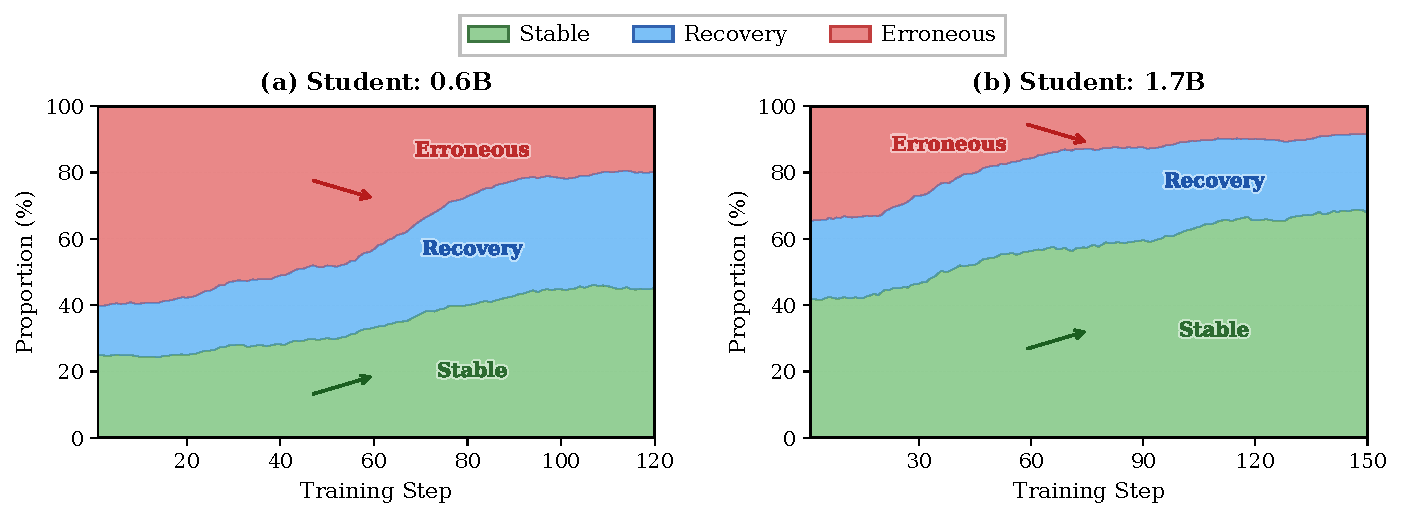
\includegraphics[width=1.0\linewidth]{pic/pattern_distribution_v23.pdf}
\caption{Distribution of three distillation patterns over training steps. At each step, all rollout trajectories are classified into Stable, Recovery, or Erroneous based on their adaptive weight dynamics, and the proportion of each pattern is reported (smoothed with a 9-step moving average).}
\label{fig:pattern_dist}
\end{figure*}

To move beyond qualitative illustration and quantify how the three distillation patterns evolve during training, we conduct a systematic classification of all multi-step trajectories at each training step. Specifically, for every rollout sample at global step $t$, we record the full sequence of adaptive weights $\{w_k\}_{k=1}^{K}$ computed by \ourmodel during that trajectory. We then classify each trajectory into one of three dominant patterns based on the overall shape of the $w_k$ sequence:

\begin{itemize}[leftmargin=1.5em, itemsep=2pt]
    \item \textbf{Stable}: Adaptive weights remain consistently high throughout the trajectory, indicating that the student stays well-aligned with the teacher across all reasoning steps.
    \item \textbf{Erroneous}: Weights are progressively suppressed and remain low by the final step, indicating persistent divergence that the student fails to correct.
    \item \textbf{Recovery}: Weights drop during intermediate steps (reflecting temporary divergence) but recover by the final step, indicating that the student successfully re-aligns after an initial deviation.
\end{itemize}

\noindent We note that a fourth logical category exists, \ie trajectories that begin aligned but \emph{degrade} toward the end (\ie early weights are high but the final weight is low). In practice, we find this pattern accounts for a negligible fraction ($<$1\%) of all trajectories, as persistent degradation without any preceding divergence signal is rare under \ourmodel's cumulative reweighting mechanism. We therefore merge these cases into the erroneous category for simplicity.
At each training step, we classify all rollout samples and compute the proportion of each pattern. Results are smoothed with a 9-step moving average for visualization clarity. Figure~\ref{fig:pattern_dist} reports the distribution over the training trajectory for both model scales.





\paragraph{Key observations.}
\textbf{(1) Stable proportion increases over training.} For both 0.6B and 1.7B, the fraction of stable trajectories grows steadily, confirming that \ourmodel progressively improves student-teacher alignment as training proceeds.
\textbf{(2) Erroneous proportion decreases consistently.} The proportion of erroneous trajectories declines substantially over training. This indicates that, as training progresses under \ourmodel, the student model becomes increasingly capable: when encountering difficult reasoning steps, it no longer falls into consecutive errors but instead recovers or avoids mistakes altogether.
\textbf{(3) Recovery grows and becomes a persistent component.} Notably, the recovery proportion is initially low (especially for the 0.6B model) and \emph{increases} over training before stabilizing at a substantial level. This reveals a meaningful progression: early in training, the student lacks the capacity to recover from divergence; once it deviates, it tends to remain erroneous. As training proceeds, the student develops the ability to self-correct after intermediate missteps, converting what would have been erroneous trajectories into recovery ones. Even at the end of training, recovery trajectories account for a significant proportion of all samples, indicating that \ourmodel's adaptive reweighting mechanism remains \emph{continuously active}.
\textbf{(4) Model capacity affects convergence speed and pattern composition.} The 1.7B model reaches a higher stable proportion faster and drives erroneous to a lower level by the end of training, while maintaining a moderate recovery proportion throughout. In contrast, the 0.6B model starts with a much higher erroneous fraction and lower recovery fraction, reflecting its initially limited ability to self-correct. As training progresses, the 0.6B model gradually develops recovery capability, but converges more slowly overall. This suggests that \ourmodel's protective suppression of erroneous signals is particularly critical for smaller models during early training.


\subsection{The Performance of Naive On-policy Distillation}
\label{app:naive_opd}

In the main experiments, our OPD baseline combines the OPD loss with GRPO (\ie $\mathcal{L} = \mathcal{L}_{\mathrm{GRPO}} + \mathcal{L}_{\mathrm{OPD}}$) as illustrated in~\cref{app:baselines}. Here we report results for \textit{naive OPD}, which uses only the token-level distillation loss without any RL reward signal.

\begin{table}[h]
    \centering
    \caption{Comparison of naive OPD vs.\ OPD on the 1.7B student model.}
    \vspace{0.4em}
    \label{tab:naive_opd}
    \begingroup
    \setlength{\tabcolsep}{4pt}
    \renewcommand{\arraystretch}{1.08}
    \begin{adjustbox}{max width=0.85\textwidth}
    \begin{tabular}{lccccc}
        \toprule
        \multirow{2}{*}{\textbf{Method}}
        & \multicolumn{2}{c}{\textbf{Math}}
        & \textbf{Science}
        & \textbf{Code}
        & \multirow{2}{*}{\textbf{Average}} \\
        \cmidrule(lr){2-3} \cmidrule(lr){4-4} \cmidrule(lr){5-5}
        & AIME 2024 & AIME 2025 & GPQA & LiveCodeBench & \\
        \midrule
        naive OPD
        & 40.54\phantom{.}\scalebox{0.72}{$\pm$1.05} & 35.83\phantom{.}\scalebox{0.72}{$\pm$1.11} & 28.96\phantom{.}\scalebox{0.72}{$\pm$0.58} & 29.81\phantom{.}\scalebox{0.72}{$\pm$0.74} & 33.79 \\
        OPD 
        & 43.86\phantom{.}\scalebox{0.72}{$\pm$1.23} & 37.04\phantom{.}\scalebox{0.72}{$\pm$1.31} & 31.73\phantom{.}\scalebox{0.72}{$\pm$0.55} & 32.45\phantom{.}\scalebox{0.72}{$\pm$0.93} & 36.27 \\
        \midrule
        \ourmodel (w/o GRPO)
        & 48.87\phantom{.}\scalebox{0.72}{$\pm$0.93} & 39.73\phantom{.}\scalebox{0.72}{$\pm$1.02} & 35.89\phantom{.}\scalebox{0.72}{$\pm$0.62} & 38.62\phantom{.}\scalebox{0.72}{$\pm$0.71} & 40.78 \\
        \textbf{\ourmodel}
        & \textbf{50.83}\phantom{.}\scalebox{0.72}{$\pm$1.15} & \textbf{41.72}\phantom{.}\scalebox{0.72}{$\pm$1.24} & \textbf{38.72}\phantom{.}\scalebox{0.72}{$\pm$0.73} & \textbf{40.63}\phantom{.}\scalebox{0.72}{$\pm$0.91} & \textbf{42.98} \\
        \bottomrule
    \end{tabular}
    \end{adjustbox}
    \endgroup
\end{table}





As shown in~\cref{tab:naive_opd}, naive OPD underperforms the OPD baseline by 2.48 points on average (33.79 vs.\ 36.27). Without the outcome-level reward signal from GRPO, the student relies entirely on dense teacher supervision for learning. However, as analyzed in~\cref{sec:failure_uniform_opd},  OPD applies uniform distillation across all steps including those corrupted by tool-induced state drift. In the absence of GRPO's reward-driven exploration, the model lacks an independent signal to distinguish successful from failed trajectories, making it more susceptible to the compounding error problem.

More notably, comparing the two pure distillation variants, naive OPD (33.79) vs.\ \ourmodel w/o GRPO (40.78), reveals that our step-wise reweighting alone accounts for a +6.99 (+20.69\%) improvement without any RL reward signal. This confirms that the core benefit of \ourmodel stems from the adaptive step-wise reweighting mechanism rather than from the RL component. GRPO provides complementary gains (+2.20 on top of step-wise OPD), but the reweighting mechanism remains the primary driver of performance improvement. These results also suggest that step-wise reweighting and GRPO address orthogonal aspects of the training challenge: the former stabilizes dense supervision under state drift, while the latter provides sparse outcome-level exploration signals.
